
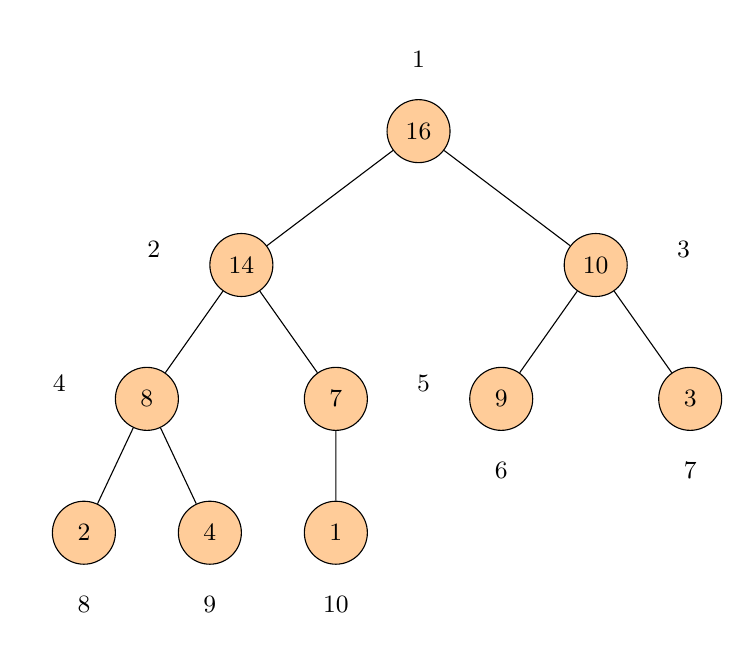
\begin{tikzpicture}[
    every node/.style={circle, draw, fill=orange!40, minimum size=8mm, font=\small},
    level distance=17mm,
    level 1/.style={sibling distance=45mm},
    level 2/.style={sibling distance=24mm},
    level 3/.style={sibling distance=16mm},
    edge from parent/.style={draw, -}
  ]

  \node[label={[yshift=1mm]above:1}] (n1) {16}
  child { node[label={[xshift=-3mm,yshift=2mm]left:2}] (n2) {14}
      child { node[label={[xshift=-3mm,yshift=2mm]left:4}] (n4) {8}
          child { node[label={[yshift=-1mm]below:8}] (n8) {2} }
          child { node[label={[yshift=-1mm]below:9}] (n9) {4} }
        }
      child { node[label={[xshift=3mm,yshift=2mm]right:5}] (n5) {7}
          child { node[label={[yshift=-1mm]below:10}] (n10) {1} }
        }
    }
  child { node[label={[xshift=3mm,yshift=2mm]right:3}] (n3) {10}
      child { node[label={[yshift=-1mm]below:6}] (n6) {9} }
      child { node[label={[yshift=-1mm]below:7}] (n7) {3} }
    };

\end{tikzpicture}
\hspace{2cm}
% ==============================================
% Figura (b): Rappresentazione ad array con archi
% ==============================================
\begin{tikzpicture}[
    every node/.style={draw, minimum width=8mm, minimum height=8mm, font=\small},
    node distance=0mm
  ]

  % Valori dell'array
  \node (a1) {16};
  \node[right=of a1] (a2) {14};
  \node[right=of a2] (a3) {10};
  \node[right=of a3] (a4) {8};
  \node[right=of a4] (a5) {7};
  \node[right=of a5] (a6) {9};
  \node[right=of a6] (a7) {3};
  \node[right=of a7] (a8) {2};
  \node[right=of a8] (a9) {4};
  \node[right=of a9] (a10) {1};

  % Indici sopra, ben distanziati dagli archi
  \foreach \i in {1,...,10}{
      \node[draw=none, above=7mm of a\i, font=\small] {\i};
    }

  % Archi genitore-figlio: curvatura proporzionale alla distanza tra i nodi
  % padre 1 -> figli 2,3
  \draw[-{Latex[length=2mm]}] (a1.north) to[bend left=25] (a2.north);
  \draw[-{Latex[length=2mm]}] (a1.north) to[bend left=45] (a3.north);

  % padre 2 -> figli 4,5
  \draw[-{Latex[length=2mm]}] (a2.north) to[bend left=25] (a4.north);
  \draw[-{Latex[length=2mm]}] (a2.north) to[bend left=45] (a5.north);

  % padre 3 -> figli 6,7
  \draw[-{Latex[length=2mm]}] (a3.north) to[bend left=25] (a6.north);
  \draw[-{Latex[length=2mm]}] (a3.north) to[bend left=45] (a7.north);

  % padre 4 -> figli 8,9
  \draw[-{Latex[length=2mm]}] (a4.north) to[bend left=25] (a8.north);
  \draw[-{Latex[length=2mm]}] (a4.north) to[bend left=45] (a9.north);

  % padre 5 -> figlio 10
  \draw[-{Latex[length=2mm]}] (a5.north) to[bend left=45] (a10.north);

\end{tikzpicture}